
\documentclass[12pt,a4paper]{article}
\usepackage[a4paper,margin=2.25cm]{geometry}
\usepackage{graphicx}
\usepackage{float}
\usepackage{booktabs}
\usepackage{array}
\usepackage{longtable}
\usepackage{tabularx}
\usepackage{xcolor}
\usepackage{hyperref}
\usepackage{caption}
\usepackage{subcaption}
\usepackage{enumitem}
\usepackage{amsmath}
\usepackage{microtype}
\hypersetup{colorlinks=true, linkcolor=blue!45!black, urlcolor=blue!45!black, citecolor=blue!45!black}
\renewcommand{\contentsname}{Cuprins}
\renewcommand{\figurename}{Figura}
\renewcommand{\tablename}{Tabelul}
\renewcommand{\arraystretch}{1.18}
\setlist[itemize]{leftmargin=1.2em,itemsep=0.2em,topsep=0.25em}
\setlist[enumerate]{leftmargin=1.4em,itemsep=0.2em,topsep=0.25em}
\newcommand{\score}[1]{\textbf{#1}}

\begin{document}

\begin{titlepage}
\centering
\vspace*{1.2cm}
{\Large Universitatea Politehnica din București\\[0.25em]
Facultatea de Automatică și Calculatoare\\[0.25em]
Seria CC}\par
\vspace{2.5cm}
{\Huge\bfseries Tema 1 -- Introducere în Machine Learning\par}
\vspace{0.4cm}
{\Large Documentație: analiză, preprocesare, regresie și clasificare}\par
\vspace{2.2cm}
\begin{tabular}{rl}
Student: & Potop Horia-Ioan \\
Grupa: & 333AA \\
An: & 2026 \\
\end{tabular}
\vfill
\begin{minipage}{0.86\textwidth}
\end{minipage}
\end{titlepage}

\setlength{\textfloatsep}{8pt}
\setlength{\floatsep}{8pt}
\setlength{\intextsep}{8pt}
\captionsetup[figure]{font=small,skip=4pt}
\tableofcontents
\newpage

\section{Introducere și obiective}
Tema are două direcții principale: prezicerea salariului, ca problemă de regresie, și prezicerea clasei \texttt{vacation}, ca problemă de clasificare multi-clasă. Documentația nu este doar o listă de modele rulate, ci o justificare a pașilor care au dus de la soluții simple, ușor de verificat, la modele mai robuste pentru distribuția din testul privat.

Cerințele urmărite în raport sunt: analiză exploratorie pentru variabile numerice și categorice, tratarea valorilor lipsă și a valorilor extreme, baseline-uri obligatorii pentru regresie și clasificare, evaluări cu metricile cerute, comparații între modele și un jurnal al încercărilor relevante. Pentru arhiva de surse, notebook-ul \texttt{main.ipynb} păstrează codul cu care au fost generate tabelele, graficele, modelele și submisiile.

\section{Descrierea setului de date}
Setul de antrenare conține 64.000 de exemple, setul local de test/validare conține 16.000 de exemple, iar testul privat Kaggle conține 16.000 de exemple fără coloanele țintă. În notebook, datele au fost păstrate în aceeași structură pentru cele două task-uri, dar cu ținte și reguli de evitare a leakage-ului diferite.

\begin{table}[H]
\centering
\caption{Structura generală a datelor folosite în temă}
\begin{tabular}{p{0.27\textwidth}p{0.18\textwidth}p{0.45\textwidth}}
\toprule
Coloană / grup & Tip & Rol în analiză \\
\midrule
\texttt{experience\_years}, \texttt{skills\_count}, \texttt{certifications}, \texttt{total\_days\_worked}, \texttt{aggregated\_score} & numeric & Variabile explicative pentru ambele probleme; unele au distribuții cu cozi lungi sau valori speciale. \\
\texttt{job\_title}, \texttt{company\_size}, \texttt{education\_level}, \texttt{industry}, \texttt{remote\_work}, \texttt{location} & categoric & Variabile care descriu contextul profesional; utile mai ales în combinații și în encodări. \\
\texttt{salary} & numeric & Ținta pentru regresie; nu se folosește ca predictor în clasificare. \\
\texttt{vacation} & categoric & Ținta pentru clasificare; nu se folosește ca predictor în regresie. \\
\bottomrule
\end{tabular}
\end{table}

\section{Analiza exploratorie a datelor}
\subsection{Variabile numerice}
Primul pas a fost inspectarea statisticilor descriptive pentru coloanele numerice. Scopul nu a fost doar detectarea valorilor extreme, ci și identificarea variabilelor care pot induce overfit sau care pot fi redundante.

\begin{table}[H]
\centering
\caption{Statistici descriptive pentru principalele variabile numerice din train}
\resizebox{\textwidth}{!}{%
\begin{tabular}{lrrrrrrrr}
\toprule
Variabilă & count & mean & std & min & Q1 & mediană & Q3 & max \\
\midrule
\texttt{experience\_years} & 64000 & 9.97 & 6.05 & 0.00 & 5.00 & 10.00 & 15.00 & 20.00 \\
\texttt{skills\_count} & 64000 & 11.60 & 10.74 & 1.00 & 5.00 & 10.00 & 15.00 & 69.00 \\
\texttt{certifications} & 64000 & 2.51 & 1.71 & 0.00 & 1.00 & 3.00 & 4.00 & 5.00 \\
\texttt{salary} & 64000 & 145683.57 & 37384.76 & 31867.00 & 119209.75 & 143299.00 & 169582.25 & 333046.00 \\
\texttt{total\_days\_worked} & 64000 & 2393.51 & 1452.04 & -1.00 & 1200.00 & 2400.00 & 3600.00 & 4800.00 \\
\texttt{aggregated\_score} & 64000 & 0.00 & 1.00 & -4.80 & -0.67 & 0.00 & 0.68 & 4.22 \\
\bottomrule
\end{tabular}%
}
\end{table}

\begin{figure}[htbp]
\centering
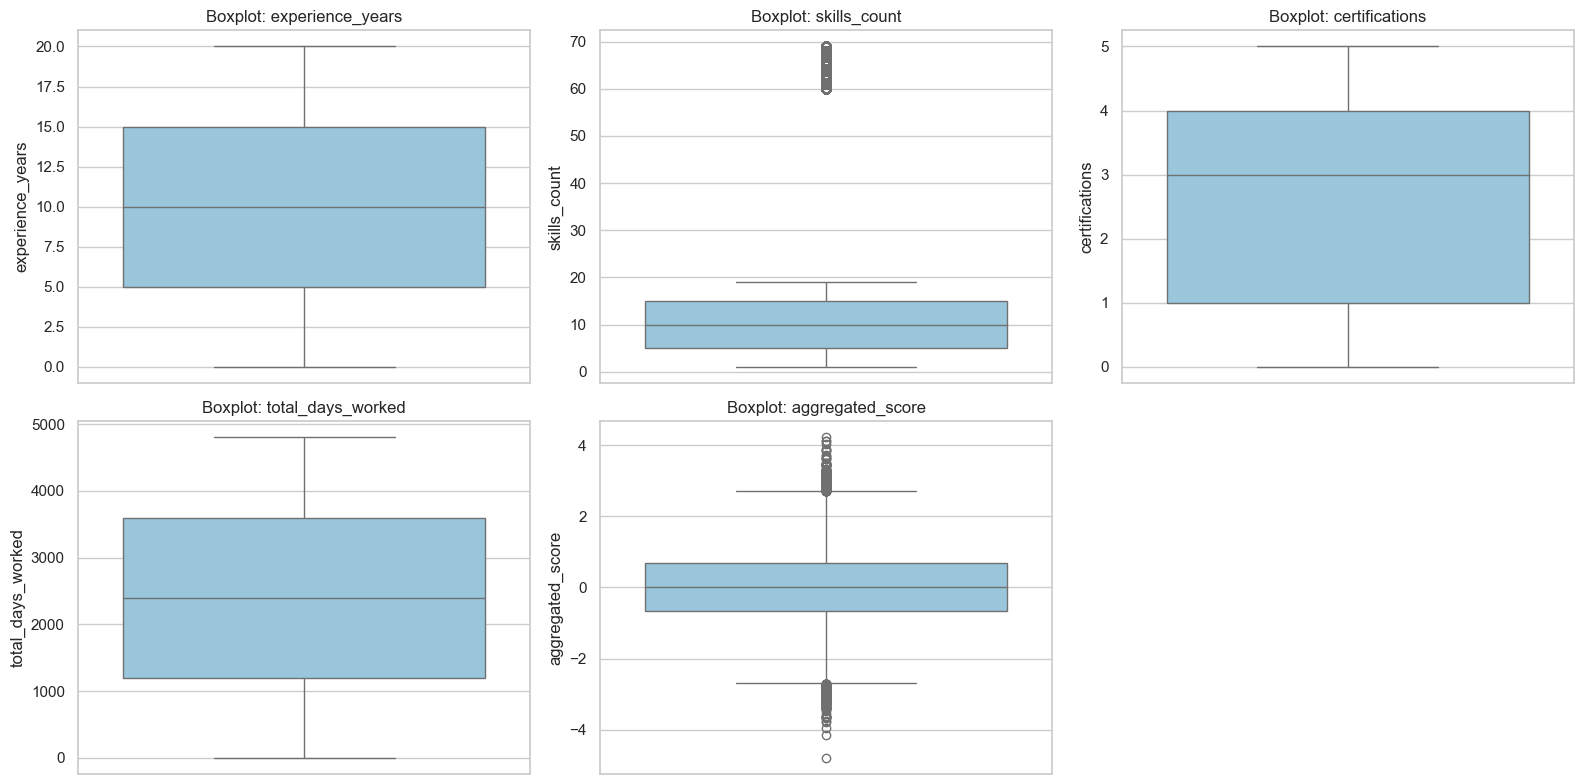
\includegraphics[width=0.74\textwidth]{figures/001_numeric_boxplots.png}
\caption{Boxplot-uri pentru variabilele numerice principale. Se observă coada lungă pentru \texttt{skills\_count}, valorile extreme din \texttt{aggregated\_score} și valoarea specială \texttt{-1} din \texttt{total\_days\_worked}.}
\end{figure}

Observațiile importante au fost următoarele. \texttt{skills\_count} are o coadă lungă, cu valori de până la 69, deși 75\% dintre exemple au cel mult 15 skill-uri. Pentru modelele liniare, astfel de valori extreme pot deplasa coeficienții și pot crește eroarea pe exemple obișnuite; pentru modelele de arbori, ele pot crea split-uri prea specifice. De aceea, în perfecționare am testat binning și indicatori de outlier, nu doar păstrarea valorii brute. \texttt{aggregated\_score} este standardizat în jurul lui 0, dar are extreme suficient de mari încât să merite analizat separat; faptul că Pearson față de salariu este aproape zero nu înseamnă că nu există semnal, ci că semnalul nu este liniar. \texttt{total\_days\_worked} este aproape echivalent cu experiența exprimată în zile și include valoarea specială \texttt{-1}, deci a fost tratat cu atenție în modelele finale și interpretat ca posibilă redundanță față de \texttt{experience\_years}.

\subsection{Valori lipsă și variabile categorice}
Singura lipsă majoră a fost la \texttt{remote\_work}: 19.153 valori lipsă în train. Această lipsă nu a fost tratată ca zgomot pur, deoarece absența informației poate fi ea însăși semnal: un rând fără informație despre remote poate proveni dintr-un tip diferit de companie sau dintr-un proces diferit de colectare. De aceea, pentru modelele de arbori a fost păstrată categoria \texttt{Missing}, iar pentru unele experimente s-a adăugat și indicatorul \texttt{remote\_work\_missing}. Pentru modelele liniare am folosit imputare/one-hot encoding, deoarece acestea nu pot lucra direct cu valori categorice lipsă.

\begin{figure}[htbp]
\centering
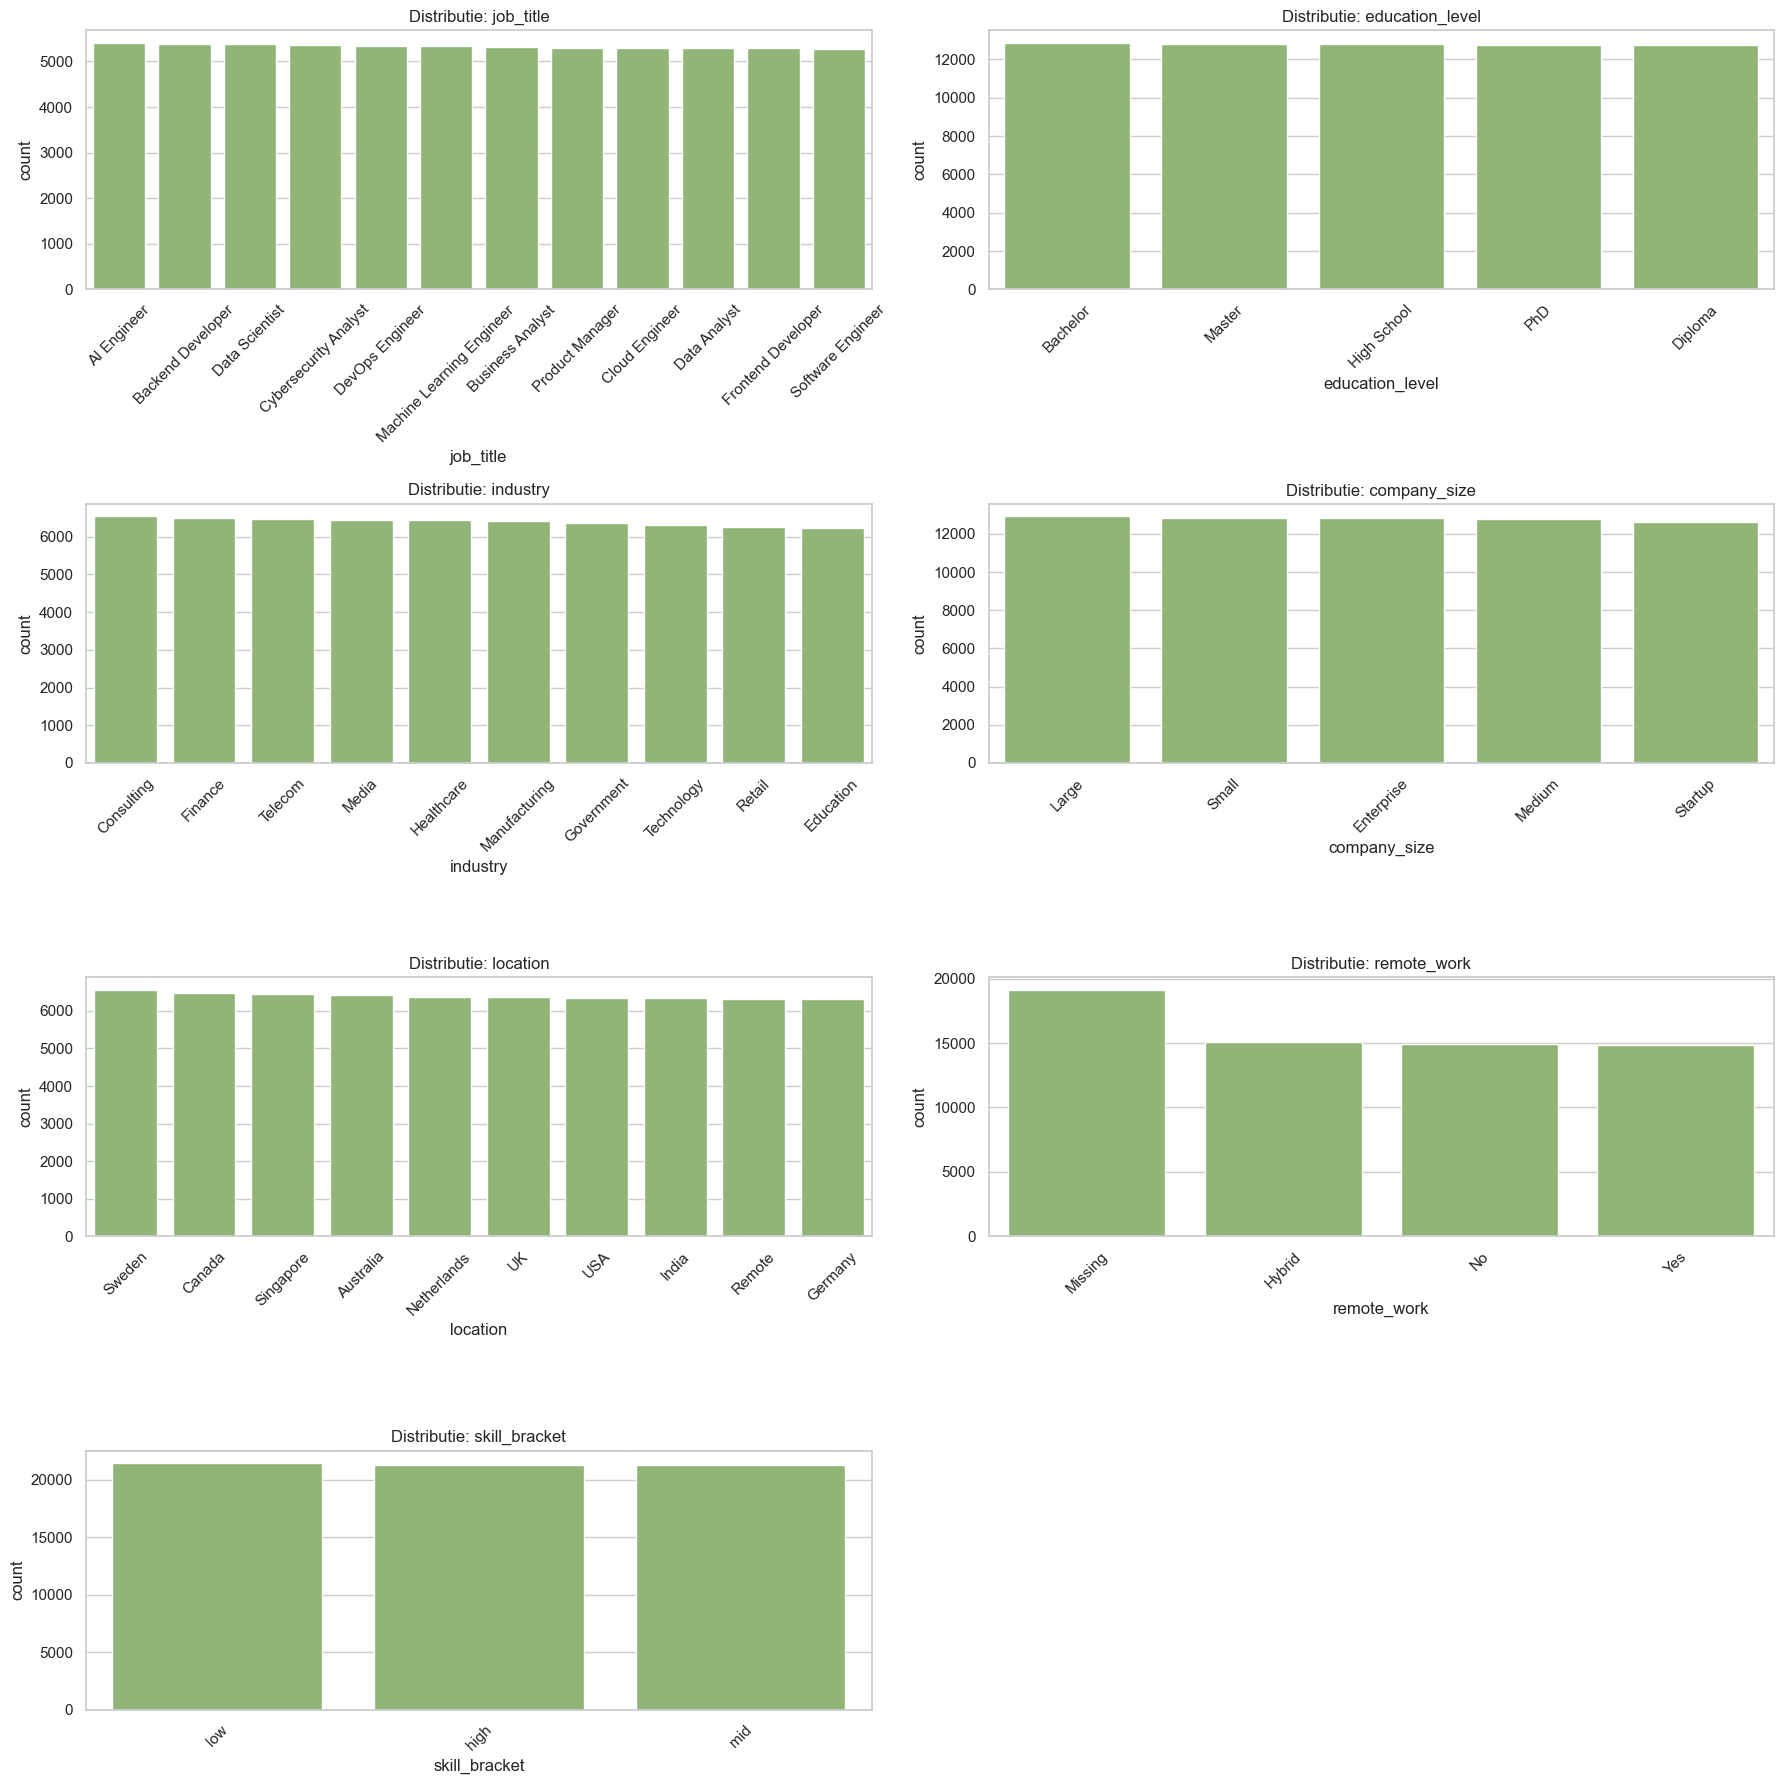
\includegraphics[width=0.74\textwidth]{figures/002_categorical_distributions.png}
\caption{Distribuțiile variabilelor categorice. Majoritatea categoriilor sunt relativ echilibrate, iar \texttt{remote\_work} are o componentă importantă de valori lipsă.}
\end{figure}

\subsection{Distribuția țintelor}
Pentru regresie, \texttt{salary} are o distribuție continuă cu valori între aproximativ 31.867 și 333.046. Distribuția are o coadă spre salarii mari, motiv pentru care transformarea \texttt{log1p} a fost utilă în modelele avansate: penalizează mai puțin disproporționat valorile mari și ajută modelul să învețe relații multiplicative. Pentru clasificare, \texttt{vacation} este dezechilibrată: clasa \texttt{No Vacation} domină, iar clasele \texttt{Large}, \texttt{Medium} și \texttt{Small} sunt mai rare. Acest dezechilibru explică de ce am raportat și F1 macro/per-clasă, nu doar accuracy; altfel un model poate părea bun doar pentru că prezice bine clasa majoritară.

\begin{table}[H]
\centering
\caption{Distribuția claselor pentru \texttt{vacation}}
\begin{tabular}{lrr}
\toprule
Clasă & Număr exemple & Procent \\
\midrule
\texttt{No Vacation} & 34686 & 54.20\% \\
\texttt{Small} & 12877 & 20.12\% \\
\texttt{Medium} & 8527 & 13.32\% \\
\texttt{Large} & 7910 & 12.36\% \\
\bottomrule
\end{tabular}
\end{table}

\begin{figure}[htbp]
\centering
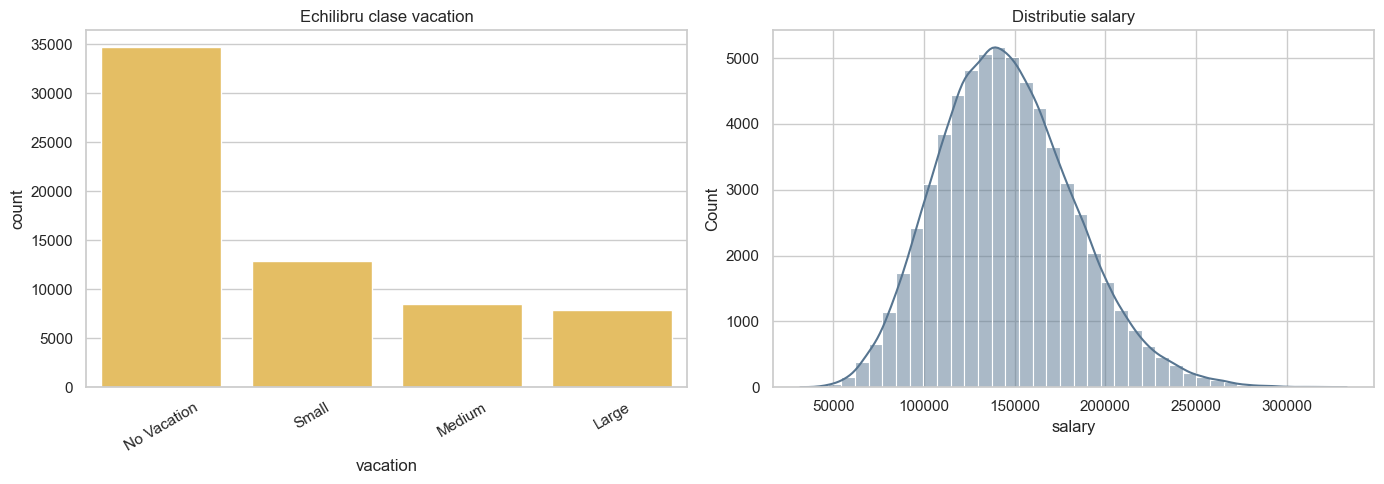
\includegraphics[width=0.74\textwidth]{figures/003_targets_distribution.png}
\caption{Distribuția țintelor: clasele \texttt{vacation} sunt dezechilibrate, iar \texttt{salary} are o distribuție unimodală cu o coadă spre salarii mari.}
\end{figure}

\subsection{Corelații și asocieri}
Pentru regresie, cele mai puternice relații numerice cu salariul apar la \texttt{experience\_years} și \texttt{total\_days\_worked}. Cele două au practic același semnal, ceea ce explică de ce, în modelele finale, \texttt{total\_days\_worked} a fost privit mai degrabă ca variabilă redundantă sau de verificare.

\begin{table}[H]
\centering
\caption{Corelații Pearson cu \texttt{salary}}
\begin{tabular}{lr}
\toprule
Variabilă & Corelație cu \texttt{salary} \\
\midrule
\texttt{experience\_years} & 0.437 \\
\texttt{total\_days\_worked} & 0.437 \\
\texttt{certifications} & 0.077 \\
\texttt{skills\_count} & 0.065 \\
\texttt{aggregated\_score} & -0.004 \\
\bottomrule
\end{tabular}
\end{table}

\begin{figure}[htbp]
\centering
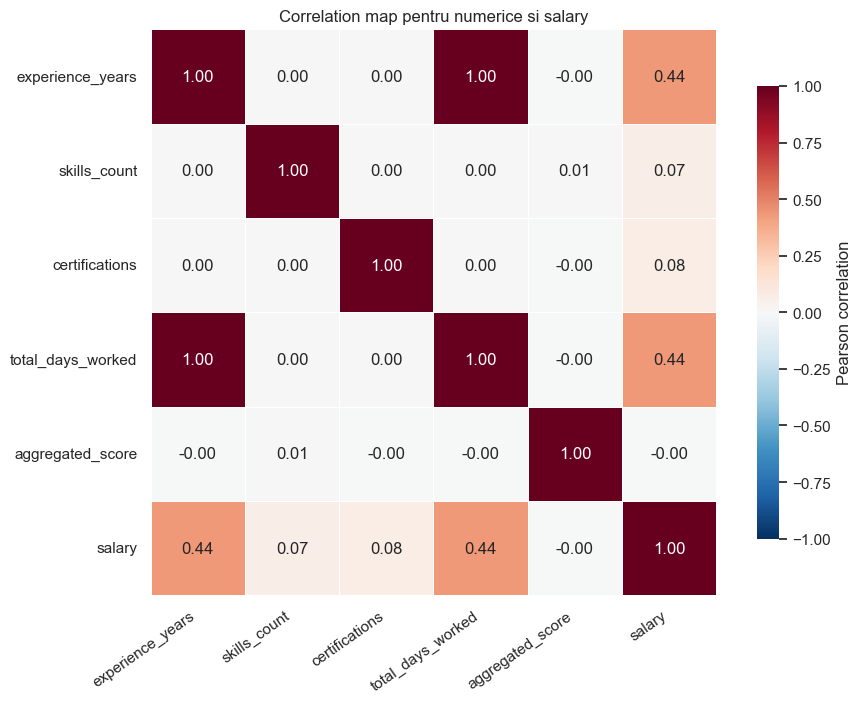
\includegraphics[width=0.74\textwidth]{figures/004_numeric_correlation_heatmap.png}
\caption{Heatmap Pearson pentru variabilele numerice și \texttt{salary}. \texttt{experience\_years} și \texttt{total\_days\_worked} sunt aproape redundante și au cea mai clară relație liniară cu salariul.}
\end{figure}

Pentru clasificare, analiza nu s-a limitat la corelații numerice. Pentru variabilele categorice s-au folosit asocieri de tip Cramer's V / chi-square, deoarece ținta \texttt{vacation} este categorică. Această analiză este mai potrivită decât Pearson pentru categorice, fiindcă măsoară asocierea dintre distribuții de clase. Dacă o variabilă are asociere mică individual, ea poate rămâne totuși utilă în combinații, de exemplu rol + locație sau educație + rol. Din acest motiv, la regresie am folosit și target encoding pe interacțiuni, iar la clasificare am preferat modele de boosting care pot combina automat mai multe split-uri slabe.

\begin{figure}[htbp]
\centering
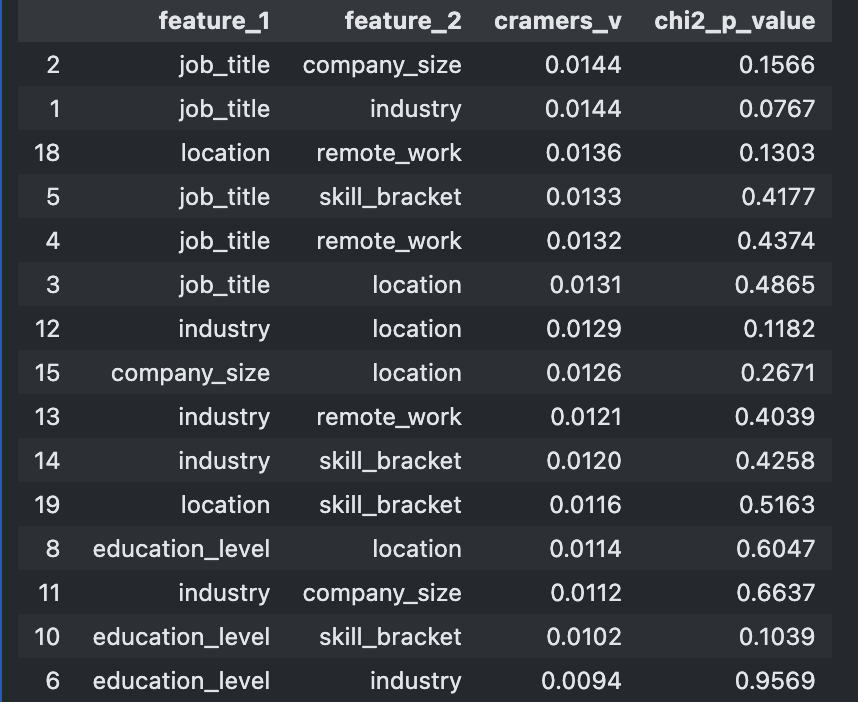
\includegraphics[width=0.74\textwidth]{figures/005_categorical_association.png}
\caption{Heatmap Cramer's V pentru variabilele categorice și \texttt{vacation}. Graficul evidențiază asocierile utile pentru clasificare și posibilele redundanțe între categorice.}
\end{figure}

\section{Preprocesare}
\subsection{Decizii comune}
Au fost aplicate câteva reguli comune pentru ambele probleme. Coloana \texttt{id} nu a fost folosită ca predictor, fiind doar identificator. Valorile lipsă din categorice au fost înlocuite cu \texttt{Missing}; numericelor li s-a aplicat imputare cu mediană când modelul cerea date complet numerice, deoarece mediana este mai robustă decât media la outlieri. Pentru modelele liniare, variabilele categorice au fost transformate prin one-hot encoding și numericile au fost standardizate, deoarece regularizarea Ridge/Lasso depinde de scara variabilelor. Pentru modelele bazate pe arbori, standardizarea nu a fost necesară, dar s-au folosit transformări care izolează distribuțiile problematice, cum ar fi binning pentru scoruri cu extreme sau indicatori pentru valori lipsă.

\subsection{Preprocesarea pentru regresie}
La regresie s-a evitat folosirea țintei de clasificare ca predictor. În varianta de bază, pipeline-ul a folosit one-hot encoding pentru categorice și imputare/standardizare pentru numerice, astfel încât modelele liniare să fie corect antrenate.

În perfecționare au fost introduse treptat transformări mai specializate: \texttt{log1p} pe salariu, target encoding cu K-Fold pentru categorice și interacțiuni, ponderi obținute din adversarial validation, pseudo-labeling pe testul privat și seed ensembling. Pentru \texttt{aggregated\_score} s-au testat variante cu păstrarea valorii brute, binning în cuantile și eliminarea valorii brute. Varianta finală a păstrat ideea de binning și a combinat doar acele ajustări care au scăzut scorul public.

\subsection{Preprocesarea pentru clasificare}
La clasificare, \texttt{salary} a fost exclus pentru a evita leakage-ul: în testul privat nu este disponibil și ar transforma problema într-una nerealistă. S-au folosit aceleași tratamente generale pentru lipsuri și categorice, dar metricile și scopul au fost diferite. Din cauza dezechilibrului între clase, modelele au fost analizate atât prin accuracy, cât și prin precision, recall și F1 pe clase.

Pentru perfecționarea clasificării, s-au testat variante de arbori și gradient boosting: Decision Tree cu hiperparametri variați, Random Forest / ExtraTrees cu ponderare, CatBoost nativ pe categorice, LightGBM multiclass și HistGradientBoosting. În plus, s-a folosit K-Fold pentru a verifica dacă scorul local este stabil, nu doar o întâmplare a splitului.

\section{Regresie: baseline și perfecționare}
\subsection{Baseline obligatoriu: regresie liniară}
Baseline-ul de regresie a pornit de la \texttt{LinearRegression}. Apoi au fost testate regularizări Ridge, Lasso și ElasticNet, cu mai multe valori pentru hiperparametri. Această etapă a fost utilă pentru a vedea cât din problemă poate fi rezolvată prin relații aproape liniare.

\begin{table}[H]
\centering
\caption{Modele liniare și regularizate pentru regresie}
\resizebox{\textwidth}{!}{%
\begin{tabular}{lrrrrr}
\toprule
Model & Train MSE & Test MSE & RMSE & MAE & $R^2$ \\
\midrule
LinearRegression baseline & $5.5605\cdot10^7$ & $5.4936\cdot10^7$ & 7411.91 & 5731.12 & 0.9602 \\
Ridge $\alpha=1$ & $5.5605\cdot10^7$ & $5.4937\cdot10^7$ & 7411.96 & 5731.14 & 0.9602 \\
Ridge $\alpha=10$ & $5.5606\cdot10^7$ & $5.4942\cdot10^7$ & 7412.29 & 5731.15 & 0.9602 \\
Lasso $\alpha=0.1$ & $5.5605\cdot10^7$ & $5.4936\cdot10^7$ & 7411.89 & 5731.11 & 0.9602 \\
\textbf{Lasso $\alpha=1.0$} & $5.5605\cdot10^7$ & \score{$5.4935\cdot10^7$} & \score{7411.82} & \score{5731.04} & \score{0.9602} \\
Lasso $\alpha=10$ & $5.5634\cdot10^7$ & $5.4966\cdot10^7$ & 7413.90 & 5732.70 & 0.9602 \\
ElasticNet $\alpha=0.01$, $l1=0.75$ & $5.6215\cdot10^7$ & $5.5512\cdot10^7$ & 7450.62 & 5752.57 & 0.9598 \\
\bottomrule
\end{tabular}%
}
\end{table}

Regularizarea nu a schimbat semnificativ rezultatul. Ridge a stabilizat coeficienții, dar nu a adus un câștig clar, ceea ce sugerează că multicoliniaritatea nu era principala problemă în baseline. Lasso cu \texttt{alpha=1.0} a fost marginal mai bun, dar diferența este foarte mică, deci nu poate fi considerată o îmbunătățire structurală. Concluzia a fost că baseline-ul liniar este solid pentru relațiile globale, mai ales experiență-salariu, dar nu poate surprinde suficient de bine interacțiunile dintre rol, educație, locație, experiență și distribuția diferită din testul privat.

\begin{figure}[htbp]
\centering
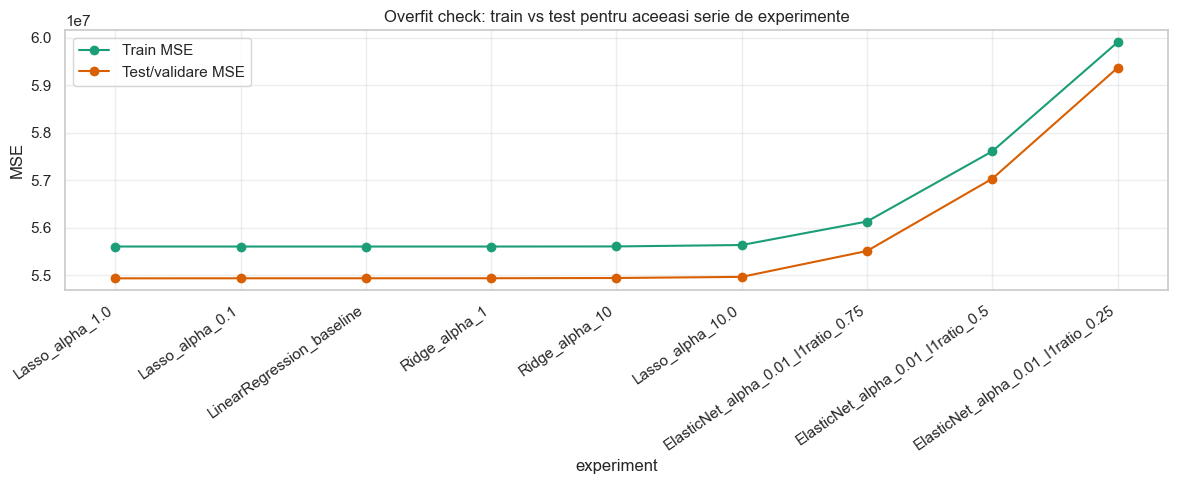
\includegraphics[width=0.74\textwidth]{figures/006_regression_baseline_curves.png}
\caption{Curbe train/test pentru modelele de regresie locale, folosite pentru a compara baseline-ul liniar cu variantele regularizate și cu etapele mai avansate.}
\end{figure}

\subsection{Adversarial validation}
O observație importantă a fost că testul privat nu are exact aceeași distribuție ca trainul local. Pentru a măsura diferența, s-a antrenat un clasificator care încearcă să distingă rândurile din train de rândurile din testul privat. Scorurile obținute au fost mari: aproximativ 0.76--0.77 AUC cu Random Forest și aproximativ 0.91 AUC în experimentele CatBoost recuperate din loguri. Acest rezultat a confirmat că nu era suficient să optimizăm doar MSE-ul local.

În urma acestei analize au fost folosite ponderi adversariale în unele modele, iar ulterior pseudo-labeling, pentru ca modelul să vadă mai bine distribuția testului privat. Ideea nu a fost să memorăm leaderboard-ul, ci să corectăm diferența reală de distribuție observată în date. Important este că seed-urile au fost folosite pentru mediere și reducerea varianței, nu pentru seed hacking: nu am ales un seed izolat doar pentru că a prins un scor bun, ci am făcut ansambluri pe mai multe antrenări și am păstrat doar etapele motivate de schimbări de preprocesare/model.

\subsection{Etapele de perfecționare pentru regresie}
Perfecționarea regresiei a avut mai multe etape clare. Am păstrat în raport doar pașii care au schimbat direcția experimentelor sau au produs o îmbunătățire relevantă.

\begin{table}[H]
\centering
\caption{Jurnalul etapelor importante pentru regresie}
\small
\begin{tabularx}{\textwidth}{p{0.13\textwidth}rrrrX}
\toprule
Etapă & MSE local & RMSE & MAE & $R^2$ & Observație \\
\midrule
CatBoost pseudo & $2.8102\cdot10^7$ & 5301.17 & 4232.88 & 0.9797 & Primul salt major: target logaritmat și pseudo-labeling. \\
LGBM pseudo & $2.9070\cdot10^7$ & 5391.62 & 4307.28 & 0.9790 & Model separat, mai slab local, dar util pentru blend. \\
CatBoost+LGBM blend & $2.7984\cdot10^7$ & 5289.99 & 4225.26 & 0.9797 & Blend-ul a redus eroarea și a confirmat diversitatea modelelor. \\
LGBM seed ensemble & $2.8846\cdot10^7$ & 5370.85 & 4289.58 & 0.9791 & Scor public mai bun: media pe seed-uri a redus varianța. \\
Away blend & $2.8879\cdot10^7$ & 5373.88 & 4291.94 & 0.9791 & Ajustare mică în direcția modelului care generaliza mai bine pe leaderboard. \\
AggBins dropraw 75\% & $2.8935\cdot10^7$ & 5379.11 & 4293.96 & 0.9791 & Transformare data-centric pentru \texttt{aggregated\_score}; scor public mai bun decât seed ensemble simplu. \\
Final V2 dropcert 20\% & \score{$2.8753\cdot10^7$} & \score{5362.21} & \score{4281.30} & \score{0.9792} & Varianta finală: combinație între modelul curent cel mai bun și o variantă V2 care corectează tratamentul unor feature-uri. \\
\bottomrule
\end{tabularx}
\end{table}

\begin{figure}[htbp]
\centering
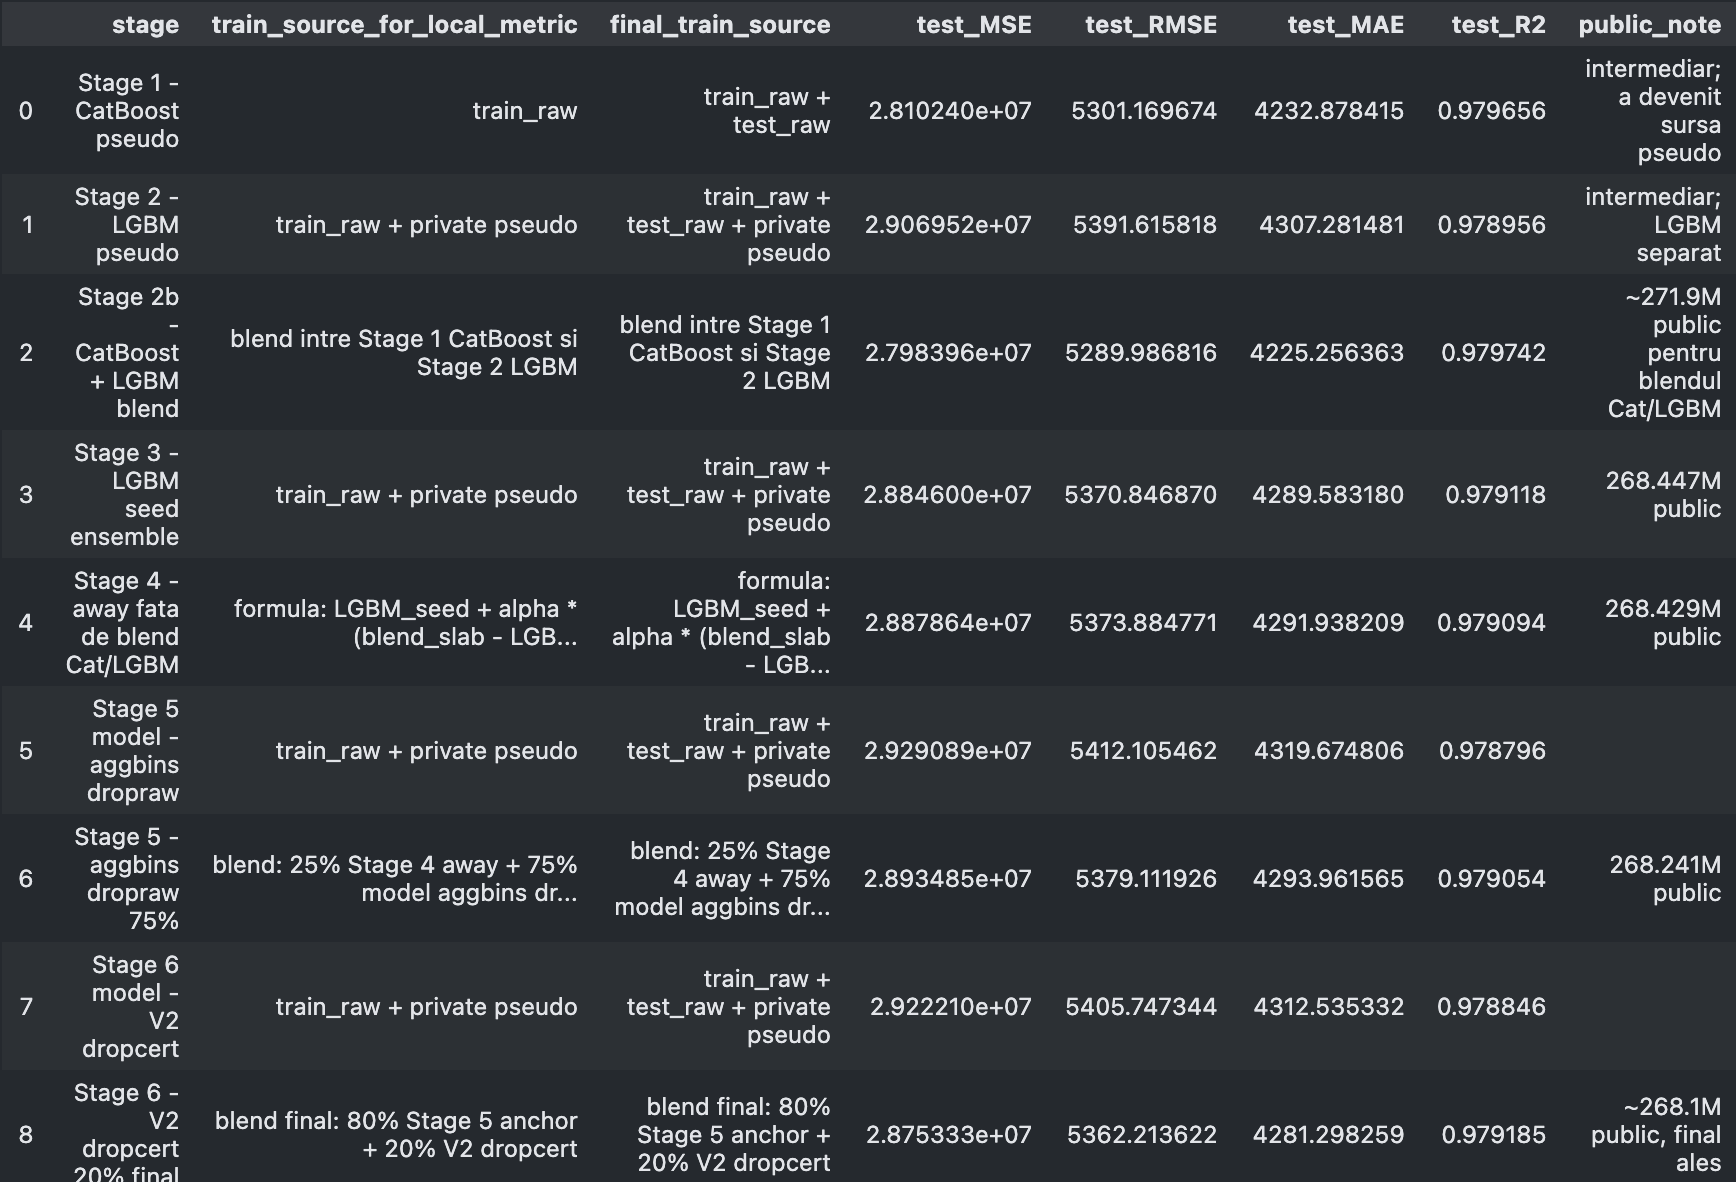
\includegraphics[width=0.74\textwidth]{figures/008_regression_perfection_stages.png}
\caption{Evoluția etapelor de perfecționare pentru regresie. Graficul/tabelul arată cum s-a trecut de la pseudo-labeling și blend-uri la seed ensembling și ajustări data-centric.}
\end{figure}

\subsection{Modelul final de regresie}
Modelul final nu este un singur algoritm izolat, ci un pipeline construit în jurul observației că distribuția din test este ușor diferită. Pașii principali au fost:

\begin{enumerate}
\item Curățarea și alinierea coloanelor între train și private test.
\item Tratarea valorilor lipsă, în special \texttt{remote\_work}, ca semnal categoric.
\item Transformarea țintei prin \texttt{log1p(salary)} și revenirea la scară prin \texttt{expm1} pentru predicții.
\item Folosirea target encoding-ului cu K-Fold pentru categorice și interacțiuni importante, astfel încât encodarea să nu vadă propria țintă a rândului curent.
\item Antrenarea de modele LightGBM pe mai multe seed-uri și medierea predicțiilor.
\item Testarea unor modele diferite, CatBoost și XGBoost, ca surse de diversitate pentru blend.
\item Ajustări data-centric: binning pentru \texttt{aggregated\_score}, analizarea \texttt{skills\_count}, \texttt{experience\_years} și \texttt{certifications}, apoi păstrarea doar a variantelor care au ajutat pe leaderboard.
\item Blend final între predicțiile care au avut comportament complementar.
\end{enumerate}

Submisia finală de regresie are 16.000 de predicții, fără valori lipsă. Distribuția predicțiilor finale a fost: medie 156.985, deviație standard 35.555, minim 42.532, mediană 155.107 și maxim 311.245. Aceste valori sunt plauzibile față de distribuția salariilor din train, ceea ce a fost o verificare suplimentară înainte de submisie.

\section{Clasificare: baseline și perfecționare}
\subsection{Baseline obligatoriu: Decision Tree}
Pentru clasificare, baseline-ul cerut a fost \texttt{DecisionTreeClassifier}. Înainte de acesta a fost inclus și un \texttt{DummyClassifier} pentru a avea o bornă minimă: dacă modelul prezice mereu clasa majoritară, accuracy-ul este aproximativ 0.542. Decision Tree a depășit clar această limită și pragul de 0.6.

\begin{table}[H]
\centering
\caption{Baseline-uri și hiperparametri pentru clasificare}
\resizebox{\textwidth}{!}{%
\begin{tabular}{lrrrr}
\toprule
Model & Train accuracy & Accuracy test & F1 macro & F1 weighted \\
\midrule
Dummy most frequent & 0.5420 & 0.5420 & 0.1757 & 0.3810 \\
DecisionTree depth 4, leaf 20 & -- & 0.6614 & -- & -- \\
DecisionTree depth 8, leaf 30 & -- & 0.7101 & -- & -- \\
\textbf{DecisionTree leaf 100} & 0.7318 & \score{0.7256} & \score{0.6686} & \score{0.7374} \\
\bottomrule
\end{tabular}%
}
\end{table}

Creșterea adâncimii arborelui a îmbunătățit rezultatul până la un punct, dar un arbore simplu rămâne limitat. Un arbore prea superficial pierde interacțiuni utile, iar unul prea adânc începe să memoreze combinații rare. Varianta cu \texttt{min\_samples\_leaf=100} a avut un echilibru mai bun, pentru că impune frunze suficient de mari. Modelele ulterioare au folosit ansambluri și boosting pentru a reduce varianța și a modela interacțiuni mai fine fără să depindă de un singur arbore.

\subsection{EDA specifică pentru clasificare}
Din cauza dezechilibrului claselor, accuracy-ul singur poate fi înșelător. De aceea, în analiza clasificării au fost urmărite și recall/F1 pe clase. Clasele \texttt{Medium} și \texttt{Small} sunt cele mai greu de separat, deoarece se suprapun mai mult în spațiul feature-urilor și au mai puține exemple decât \texttt{No Vacation}.

\begin{figure}[htbp]
\centering
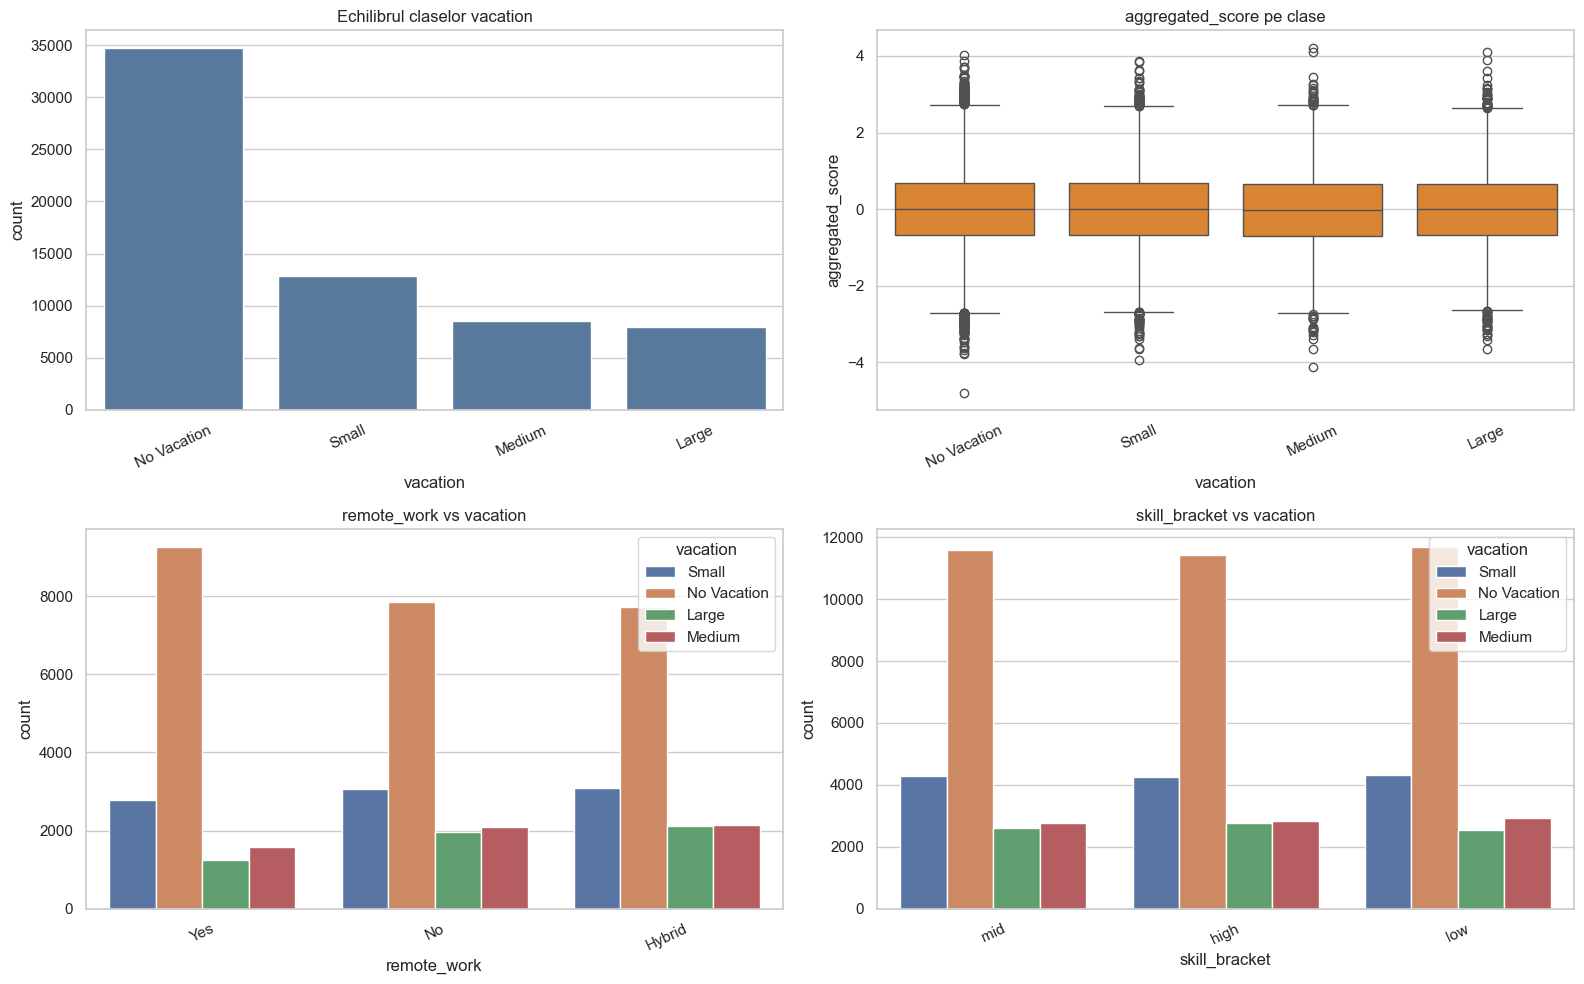
\includegraphics[width=0.74\textwidth]{figures/010_classification_eda.png}
\caption{EDA specifică pentru clasificare: balanța claselor și relația dintre \texttt{vacation} și câteva variabile numerice/categorice relevante.}
\end{figure}

\subsection{Modele încercate pentru perfecționare}
Au fost testate modele cu comportament diferit. CatBoost a fost o alegere naturală deoarece gestionează bine categoricele. LightGBM și HistGradientBoosting au fost testate pentru performanță pe date tabelare, iar ExtraTrees/RandomForest pentru robustețe și diversitate.

\begin{table}[H]
\centering
\caption{Comparație între modelele principale de clasificare}
\resizebox{\textwidth}{!}{%
\begin{tabular}{lrrrrr}
\toprule
Model & Train accuracy & Accuracy & Precision macro & Recall macro & F1 macro \\
\midrule
ExtraTrees balanced & -- & 0.7432 & -- & -- & \score{0.6818} \\
RandomForest balanced & -- & 0.7428 & -- & -- & 0.6773 \\
CatBoost V1 FE keepraw & -- & 0.7591 & -- & -- & 0.6761 \\
LightGBM multiclass & 0.7903 & 0.7603 & 0.6858 & 0.6676 & 0.6759 \\
CatBoost native & 0.7647 & 0.7606 & \score{0.6891} & \score{0.6722} & 0.6801 \\
\textbf{HistGradientBoosting final} & 0.7965 & \score{0.7611} & 0.6873 & 0.6695 & 0.6777 \\
\bottomrule
\end{tabular}%
}
\end{table}

HistGradientBoosting a fost ales ca model final după accuracy local, deși CatBoost și ExtraTrees au fost foarte apropiate sau chiar mai bune pe anumite metrici macro. Aceasta este o diferență importantă: dacă obiectivul ar fi fost exclusiv F1 macro, alegerea finală putea fi diferită. ExtraTrees ajută clasele minoritare prin randomizare și de aceea macro-F1 este competitiv, în timp ce HistGradientBoosting optimizează mai bine separarea globală și clasa majoritară. Pentru cerința temei și pentru stabilitatea locală, HistGradientBoosting a fost varianta finală de submisie.

\begin{figure}[htbp]
\centering
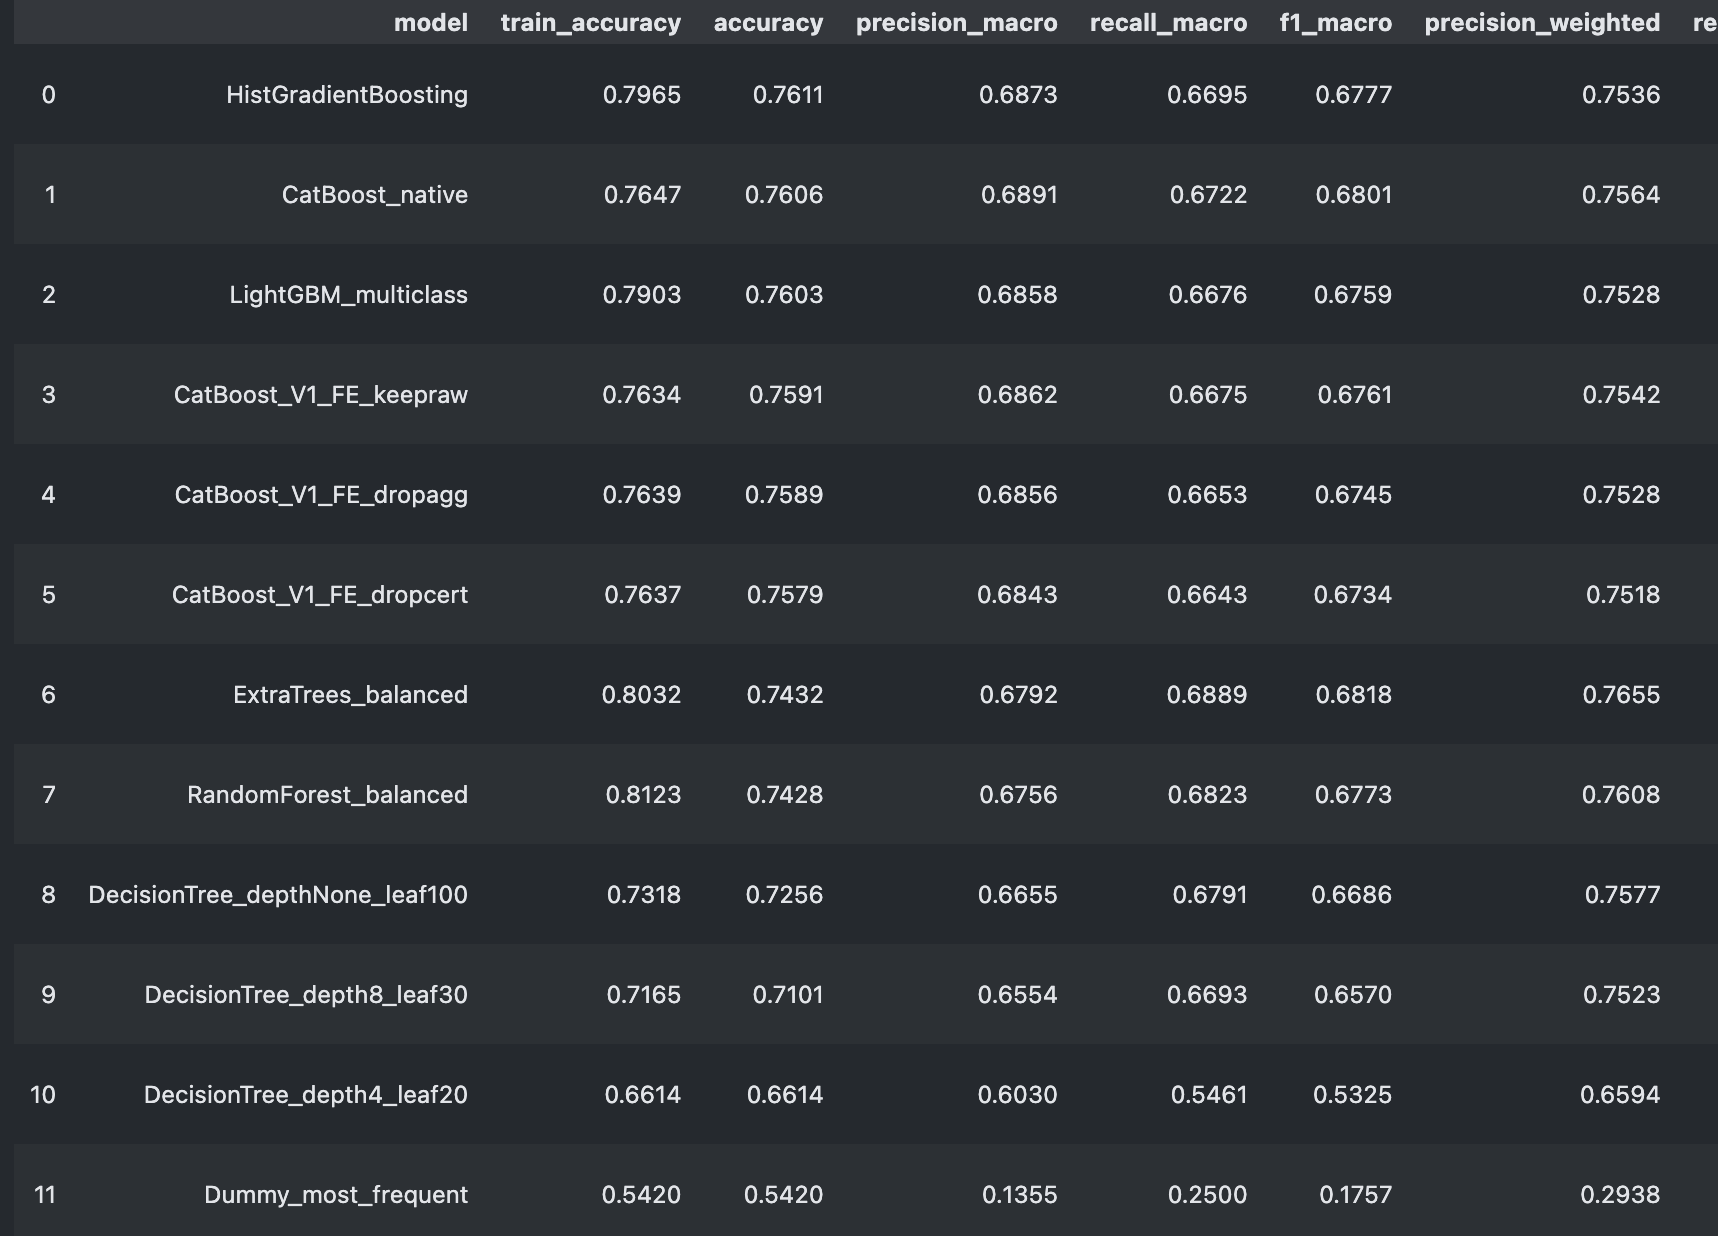
\includegraphics[width=0.74\textwidth]{figures/011_classification_model_comparison.png}
\caption{Comparație între modelele de clasificare testate, de la Decision Tree și ensemble-uri de arbori până la boosting și CatBoost.}
\end{figure}

\subsection{Evaluarea finală pentru clasificare}
Modelul final a fost evaluat prin matrice de confuzie și metrici per clasă. Clasa \texttt{No Vacation} este recunoscută cel mai bine, iar confuziile cele mai frecvente apar între \texttt{Small} și \texttt{Medium}. Acest lucru este coerent cu natura problemei: aceste clase sunt apropiate semantic și probabil împart multe profiluri similare.

\begin{table}[H]
\centering
\caption{Metrici per clasă pentru HistGradientBoosting final}
\begin{tabular}{lrrrr}
\toprule
Clasă & Precision & Recall & F1 & Support \\
\midrule
\texttt{Large} & 0.7772 & 0.7410 & 0.7587 & 1977 \\
\texttt{Medium} & 0.5434 & 0.4812 & 0.5104 & 2132 \\
\texttt{No Vacation} & 0.8737 & 0.9171 & 0.8949 & 8672 \\
\texttt{Small} & 0.5551 & 0.5387 & 0.5467 & 3219 \\
\bottomrule
\end{tabular}
\end{table}

\begin{table}[H]
\centering
\caption{Matricea de confuzie pentru HistGradientBoosting final}
\begin{tabular}{lrrrr}
\toprule
Actual / Prezis & Large & Medium & No Vacation & Small \\
\midrule
Large & 1465 & 376 & 63 & 73 \\
Medium & 364 & 1026 & 101 & 641 \\
No Vacation & 12 & 31 & 7953 & 676 \\
Small & 44 & 455 & 986 & 1734 \\
\bottomrule
\end{tabular}
\end{table}

\begin{figure}[htbp]
\centering
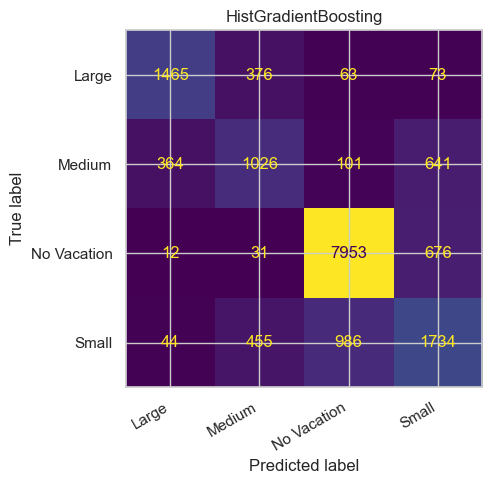
\includegraphics[width=0.74\textwidth]{figures/012_classification_confusion_matrix.png}
\caption{Matricea de confuzie pentru modelul final de clasificare. Cele mai dificile separări apar între clasele \texttt{Small} și \texttt{Medium}.}
\end{figure}

Pentru stabilitate, modelul final a fost verificat și cu 3-Fold cross-validation. Accuracy-ul pe folduri a fost 0.7600, 0.7562 și 0.7615, cu medie aproximativ 0.7592. F1 macro mediu a fost aproximativ 0.6702. Variația mică între folduri sugerează că modelul nu depinde excesiv de un singur split. Matricea de confuzie arată totuși limita principală: \texttt{No Vacation} este prezisă cel mai bine, iar \texttt{Medium} are recall mai slab deoarece se confundă des cu \texttt{Small}. Aceasta este consecința directă a dezechilibrului de clase și a suprapunerii dintre clasele intermediare.

\section{Rezultate Kaggle și fișiere finale}
Pentru regresie, cel mai bun rezultat a venit după combinația dintre seed ensembling, transformări data-centric și blend-ul final. Scorul public a coborât de la variante de aproximativ 273M la aproximativ 268M. Diferențele de la final au devenit mici, ceea ce indică faptul că partea de modelare era deja aproape saturată, iar câștigurile rămase veneau mai ales din procesarea datelor și alegerea predicțiilor de combinat.

\begin{figure}[htbp]
\centering

\includegraphics[width=0.74\textwidth]{figures/013_kaggle_regression.png}
\caption{Screenshot cu scorul final de regresie pe Kaggle.}
\end{figure}

Pentru clasificare, submisia finală generată este \texttt{submission\_classification\_final.csv}. Distribuția predicțiilor pe testul privat a fost verificată pentru a nu produce un colaps într-o singură clasă: aproximativ 34.08\% \texttt{No Vacation}, 28.26\% \texttt{Small}, 21.23\% \texttt{Medium} și 16.43\% \texttt{Large}.

\begin{figure}[htbp]
\centering

\includegraphics[width=0.74\textwidth]{figures/014_kaggle_classification.png}
\caption{Verificarea finală pentru submisia de clasificare / distribuția predicțiilor generate.}
\end{figure}

Fișierele principale de predare sunt:
\begin{itemize}
\item \texttt{main.ipynb}: notebook-ul complet, cu EDA, preprocesare, antrenare și evaluare.
\item \texttt{submission\_regression\_final.csv}: submisia finală pentru regresie.
\item \texttt{submission\_classification\_final.csv}: submisia finală pentru clasificare.
\item \texttt{regression\_csv\_selected/}: CSV-uri reprezentative pentru baseline și etapele importante de perfecționare.
\item \texttt{classification\_csv\_selected/}: rezultate, rapoarte și submisii relevante pentru clasificare.
\end{itemize}

\section{Concluzii}
Pentru regresie, cele mai mari câștiguri nu au venit dintr-un singur hiperparametru, ci din înțelegerea distribuției datelor. Adversarial validation a arătat că testul privat diferă de train, pseudo-labeling a introdus informație despre această distribuție, iar seed ensembling-ul LightGBM a redus variația. Experimentele finale cu \texttt{aggregated\_score}, binning și tratamentul unor variabile au arătat că, după ce modelul este deja puternic, micile decizii de preprocesare pot conta mai mult decât schimbarea algoritmului.

Pentru clasificare, baseline-ul Decision Tree a depășit pragurile obligatorii, dar modelele de boosting au oferit rezultate mai bune. HistGradientBoosting a avut cel mai bun accuracy local, CatBoost a fost foarte apropiat și mai bun pe unele metrici macro, iar ExtraTrees a arătat că un model mai randomizat poate ajuta clasele minoritare. Matricea de confuzie confirmă că problema rămasă este separarea claselor \texttt{Small} și \texttt{Medium}.

Dacă aș continua tema, următorii pași ar fi: o optimizare mai atentă pentru F1 macro la clasificare, calibrare de probabilități pentru clasele minoritare, o validare adversarială separată pentru clasificare și un stacked ensemble controlat pentru regresie, nu doar blend manual între CSV-uri. Totuși, pentru forma finală a temei, soluția include toate cerințele de baseline, evaluare, comparație și justificare a experimentelor.

\end{document}
